The tests were conducted using 4 nodes connected to a gateway. The nodes were placed one on each shelf of the experimental rig in order to see how the height of the shelf affects vibrations, 
similar to a tall building. The nodes were securely mounted and calibrated until they were stable enough to not be affected by small vibrations which could corrupt the actual data. 
This would also apply to a real world scenario, where the nodes would need a sturdy mounting place to properly sense relevant vibrations in the structure of the building.

We have conducted 4 test runs by setting the supply voltage for the shake table's motors at different values. The shake table was powered on for 3 seconds during each test run. The first test is performed with a still table to verify just how sensitive the sensor nodes are. Then, we simulated 3 types of vibrations generated by different movements: small vibrations obtained by swaying the test table, medium vibrations obtained by shaking the test table and large vibrations obtained by 
violently shaking the test table.

We are interested in two specific results from this experiment. First, we want to see that the sensor readings are proportional to the type of vibration applied to 
the experimental rig. Second, we want to see how the sensor readings vary in relation to height. It is known that for tall objects such as buildings, the higher you 
go, the more intense the effects of vibrations become.

In figure~\ref{fig:same-sensor} we see the accelerometer readings for the sensor placed on the lowest shelf of the experimental rig taken during each test run. The
readings show that while the table is still, the sensor is stable and does not present any relevant activity. As we start increasing the intensity of the vibrations,
more and more spikes appear in the readings and they start reverting to normal as the vibrations stop. This shows that the Sparrow v4 sensors cand reliably record 
the intensity of an event.

\begin{figure}[ht] \centering
  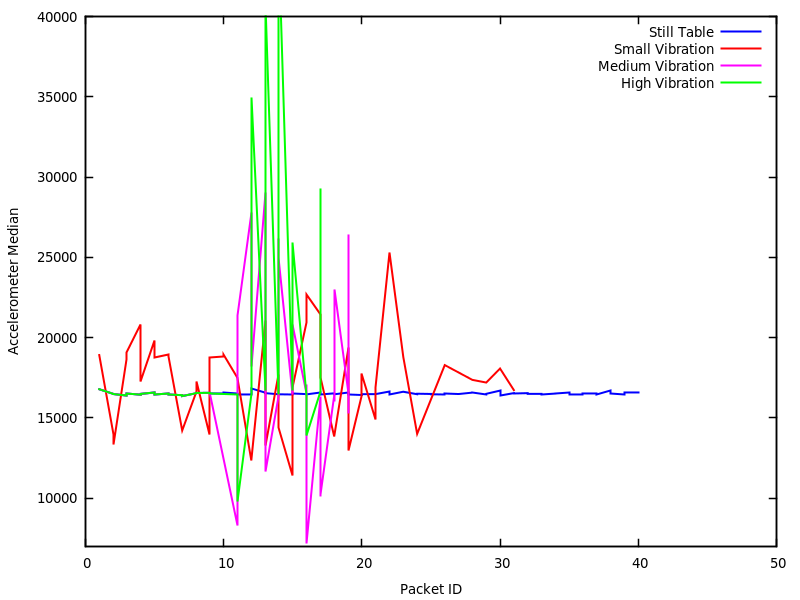
\includegraphics[width=0.5\textwidth]{img/same-sensor.png}
  \caption{Results for a sensor at different intensities}
  \label{fig:same-sensor}
\end{figure}

In figure~\ref{fig:same-level} we see the accelerometer readings for all 4 sensors taken during the same test run. The data from all the sensors shows 
that the experimental setup is experiencing vibrations. However, it can be noticed that the readings from the sensors placed near the top of the table have a 
greater amplitude. This shows that, as we theorized initially, the sensor placed closer to the top level will record a higher level of vibration and movement than 
those placed near the bottom.

\begin{figure}[ht] \centering
  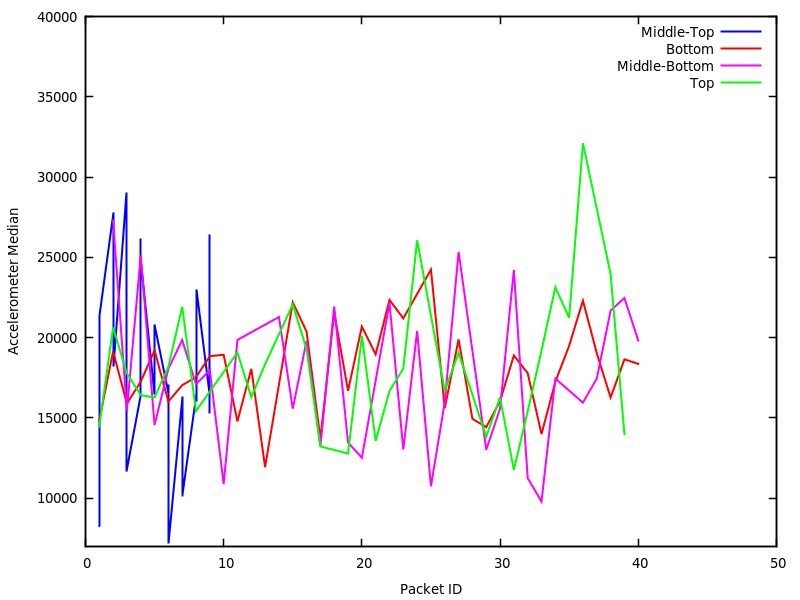
\includegraphics[width=0.5\textwidth]{img/same-level.png}
  \caption{Results for all sensors at the same intensity}
  \label{fig:same-leve}
\end{figure}

The results prove that the experimental rig is responding similar to a tall building because the lower positioned nodes gather lower amplitude values than the ones located on higher shelves 
when the table is vibrating. At the end of the simulation, when the table is no longer being shaken and it is naturaly vibrating due to previous forces, the higher positioned nodes continue 
to detect vibrations, as it should have happened in the case of a real building.
